%! Author = angela
%! Date = 24/01/24
% !TeX root = ../thesis-main.tex

\chapter{Contributions}
\label{ch:contributions}

\section{Exchange in Collektive}
\label{sec:exchange-in-collektive}


\section{DSL}
\label{sec:dsl}


\section{Plugin Extensions}
\label{sec:plugin-extensions}

\paragraph{Alignment}

\section{Incarnation}
\label{sec:incarnation}


\section{Technologies}
\label{sec:technologies}


\section{Implementation}
\label{sec:implementation}


%I suggest referencing stuff as follows: \cref{fig:random-image} or \Cref{fig:random-image}
%
%\begin{figure}
%    \centering
%    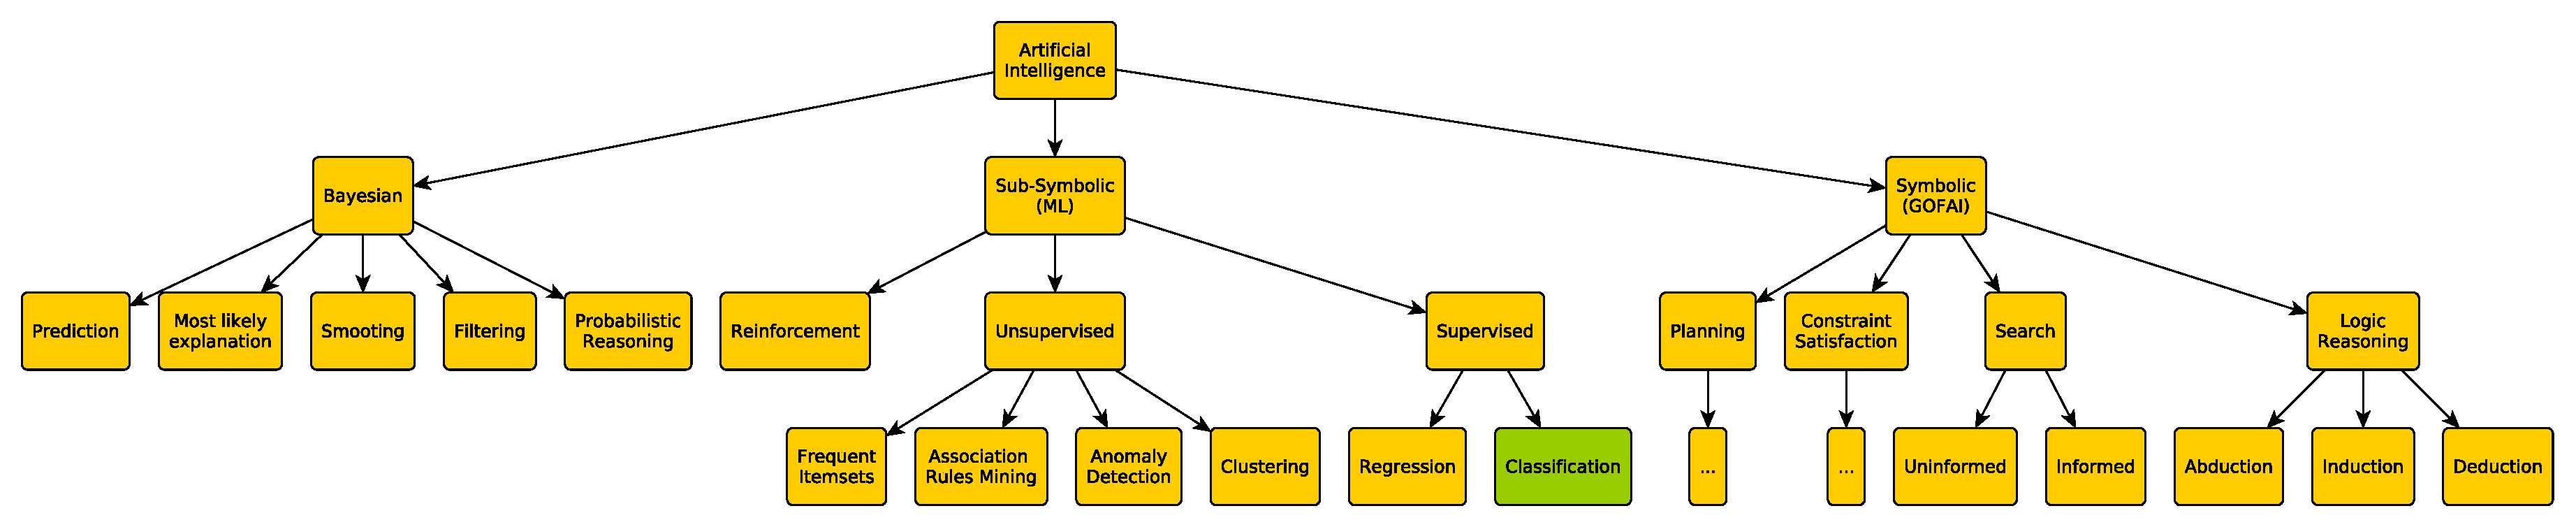
\includegraphics[width=.8\linewidth]{figures/random-image}
%    \caption{Some random image}
%    \label{fig:random-image}
%\end{figure}
%


